%%%%%%%%%%%%%%%%%
% This is an example CV created using altacv.cls (v1.1, 21 November 2016) written by
% LianTze Lim (liantze@gmail.com), based on the 
% Cv created by BusinessInsider at http://www.businessinsider.my/a-sample-resume-for-marissa-mayer-2016-7/?r=US&IR=T
% 
%% It may be distributed and/or modified under the
%% conditions of the LaTeX Project Public License, either version 1.3
%% of this license or (at your option) any later version.
%% The latest version of this license is in
%%    http://www.latex-project.org/lppl.txt
%% and version 1.3 or later is part of all distributions of LaTeX
%% version 2003/12/01 or later.
%%%%%%%%%%%%%%%%

%% If you want to use \orcid or the
%% academicons icons, add "academicons"
%% to the \documentclass options. 
%% Then compile with XeLaTeX or LuaLaTeX.
% \documentclass[10pt,a4paper,academicons]{altacv}
\documentclass[10pt,a4paper]{altacv}

%% AltaCV uses the fontawesome and academicon fonts
%% and packages. 
%% See texdoc.net/pkg/fontawecome and http://texdoc.net/pkg/academicons for full list of symbols.
%% When using the "academicons" option,
%% Compile with LuaLaTeX for best results. If you
%% want to use XeLaTeX, you may need to install
%% Academicons.ttf in your operating system's font %% folder.


% Geometría de ancho completo para página 1
\geometry{left=1cm,right=1cm,top=1cm,bottom=1cm}
% Guardar geometría de dos columnas para página 2
\newcommand{\twocolgeometry}{\newgeometry{left=1cm,right=9cm,marginparwidth=6.8cm,marginparsep=1.2cm,top=1cm,bottom=1cm}}

% Change the font if you want to.

% If using pdflatex:
\usepackage[utf8]{inputenc}
\usepackage[T1]{fontenc}
\usepackage[default]{lato}
\usepackage{enumitem} % For customizing lists
\usepackage{multicol} % Para formato de múltiples columnas
\usepackage{ragged2e} % Para justificar texto
\usepackage{pgfplots} % Para gráficos de barras
\pgfplotsset{compat=1.17}
% Colores para el gráfico de barras (paleta azul-verde)
\definecolor{colorB2B}{HTML}{1A5276}
\definecolor{colorProspeccion}{HTML}{1E8C8C}
\definecolor{colorCRM}{HTML}{48B4A0}
\definecolor{colorCierre}{HTML}{6BC9A6}
\definecolor{colorDificultades}{HTML}{8FD9B6}
\definecolor{colorPruebas}{HTML}{B5E7A0}

% Colores para el wheelchart (paleta azul-teal)
\definecolor{wheel1}{HTML}{1B4F72}
\definecolor{wheel2}{HTML}{2874A6}
\definecolor{wheel3}{HTML}{1ABC9C}
\definecolor{wheel4}{HTML}{48C9B0}
\definecolor{wheel5}{HTML}{76D7C4}
\definecolor{wheel6}{HTML}{A3E4D7}

% If using xelatex or lualatex:
% \setmainfont{Lato}

% Change the colours if you want to
\definecolor{VividPurple}{HTML}{1B4A5C}
\definecolor{SlateGrey}{HTML}{2E2E2E}
\definecolor{LightGrey}{HTML}{666666}
\colorlet{heading}{VividPurple}
\colorlet{accent}{VividPurple}
\colorlet{emphasis}{SlateGrey}
\colorlet{body}{LightGrey}

% Change the bullets for itemize and rating marker
% for \cvskill if you want to
\renewcommand{\itemmarker}{{\small\textbullet}}
\renewcommand{\ratingmarker}{\faCircle}

%% sample.bib contains your publications
% \addbibresource{sample.bib} % Comentado - no se usan publicaciones

% Redefinir cvevent para que fecha y ubicación estén más juntos
\renewcommand{\cvevent}[4]{%
  {\large\bfseries\color{emphasis}#1\par}
  \smallskip
  \textbf{\color{accent}#2}\par
  \smallskip
  {\small\faCalendar \hspace{0.5em}#3\hspace{2em}%
  \ifstrequal{#4}{}{}{\faMapMarker\hspace{0.5em}#4}\par}
  \medskip
}

% Redefinir wheelchart sin centering para poder posicionarlo manualmente
\renewcommand{\wheelchart}[3]{%
    \begingroup
    \def\innerradius{#2}%
    \def\outerradius{#1}%
    \pgfmathsetmacro{\totalnum}{0}%
    \foreach \value/\colour/\name in {#3} {%
        \pgfmathparse{\value+\totalnum}%
        \global\let\totalnum=\pgfmathresult%
    }%
    \begin{tikzpicture}
      \pgfmathsetmacro{\wheelwidth}{\outerradius-\innerradius}
      \pgfmathsetmacro{\midradius}{(\outerradius+\innerradius)/2}
      \begin{scope}[rotate=-90]
      \pgfmathsetmacro{\cumnum}{0}
      \foreach \value/\width/\colour/\name in {#3} {
            \pgfmathsetmacro{\newcumnum}{\cumnum + \value/\totalnum*360}
            \pgfmathsetmacro{\percentage}{\value/\totalnum*100}
            \pgfmathsetmacro{\midangle}{-(\cumnum+\newcumnum)/2}
            \pgfmathparse{(-\midangle>180?"west":"east")} \edef\textanchor{\pgfmathresult}
            \pgfmathparse{(-\midangle>180?"flush left":"flush right")} \edef\textalign{\pgfmathresult}
            \pgfmathsetmacro\labelshiftdir{1-2*(-\midangle<180)}
            \filldraw[draw=white,fill=\colour] (-\cumnum:\outerradius) arc (-\cumnum:-(\newcumnum):\outerradius) --
            (-\newcumnum:\innerradius) arc (-\newcumnum:-(\cumnum):\innerradius) -- cycle;
            \draw [*-,thin,emphasis] node [append after command={(\midangle:\midradius pt) -- (\midangle:\outerradius + 1ex) -- (\tikzlastnode)}] at (\midangle:\outerradius + 1ex) [xshift=\labelshiftdir*0.5cm,inner sep=1ex, outer sep=0pt, text width=\width,anchor=\textanchor,align=\textalign,font=\small,text=body]{\name};
            \global\let\cumnum=\newcumnum
        }
      \end{scope}
    \end{tikzpicture}\par
    \endgroup
}

\begin{document}
\name{Ana María \newline Albarracín Noreña}
  \tagline{ Ejecutiva Comercial B2B}
% Cropped to square from https://en.wikipedia.org/wiki/Marissa_Mayer#/media/File:Marissa_Mayer_May_2014_(cropped).jpg, CC-BY 2.0
\photo{5.5cm}{me}
% Personal info without bullet points
\personalinfo{%
  \textcolor{accent}{\faEnvelope}\hspace{0.5em}amalbarracin5@gmail.com \\
  \textcolor{accent}{\faPhone}\hspace{0.5em}(+57) 312 825 5775 \\
  \textcolor{accent}{\faLinkedin}\hspace{0.5em}linkedin.com/in/ana-maria-albarracin \\
  \textcolor{accent}{\faMapMarker}\hspace{0.5em}Tarjeta profesional: 26272
}

\makecvheader

\cvsection{Habilidades Comerciales} 
\begin{center}
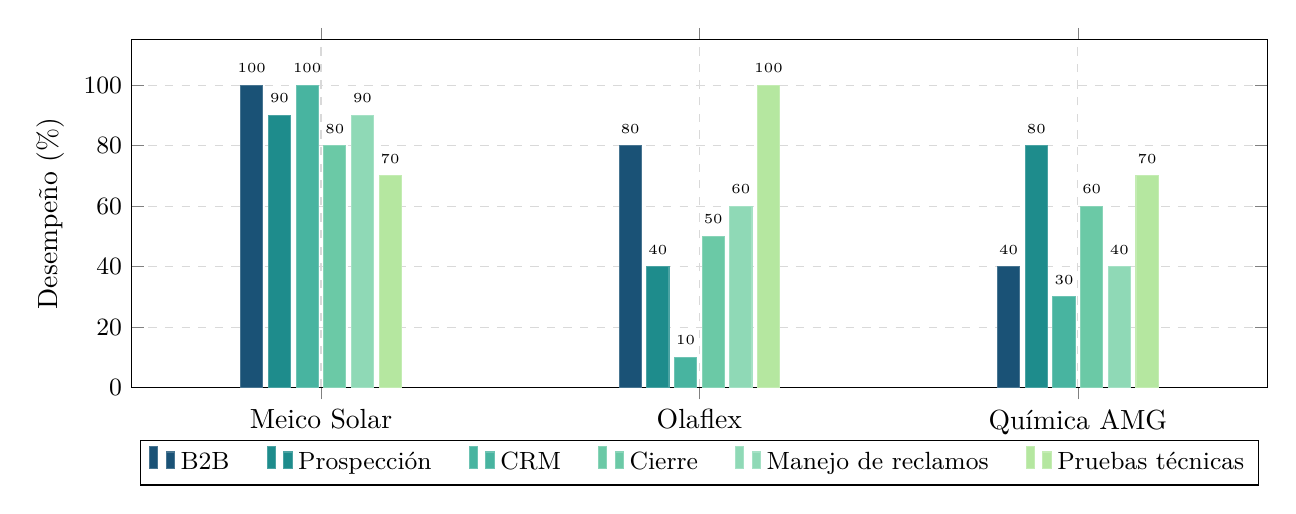
\begin{tikzpicture}
\begin{axis}[
    ybar,
    width=16cm,
    height=6cm,
    bar width=8pt,
    ylabel={Desempeño (\%)},
    ymin=0,
    ymax=115,
    ytick={0,20,40,60,80,100},
    symbolic x coords={Meico Solar, Olaflex, Química AMG},
    xtick=data,
    x tick label style={font=\normalsize},
    y tick label style={font=\small},
    ylabel style={font=\normalsize},
    legend style={
        at={(0.5,-0.15)},
        anchor=north,
        legend columns=6,
        font=\small,
        /tikz/every even column/.append style={column sep=0.4cm}
    },
    nodes near coords,
    nodes near coords style={font=\tiny, above},
    every node near coord/.append style={yshift=1pt},
    enlarge x limits=0.25,
    grid=major,
    grid style={dashed, gray!30},
]
% B2B - Azul oscuro
\addplot[fill=colorB2B, draw=colorB2B!80] coordinates {
    (Meico Solar,100) (Olaflex,80) (Química AMG,40)
};
% Prospección
\addplot[fill=colorProspeccion, draw=colorProspeccion!80] coordinates {
    (Meico Solar,90) (Olaflex,40) (Química AMG,80)
};
% CRM
\addplot[fill=colorCRM, draw=colorCRM!80] coordinates {
    (Meico Solar,100) (Olaflex,10) (Química AMG,30)
};
% Cierre
\addplot[fill=colorCierre, draw=colorCierre!80] coordinates {
    (Meico Solar,80) (Olaflex,50) (Química AMG,60)
};
% Manejo de incidencias y reclamos
\addplot[fill=colorDificultades, draw=colorDificultades!80] coordinates {
    (Meico Solar,90) (Olaflex,60) (Química AMG,40)
};
% Pruebas
\addplot[fill=colorPruebas, draw=colorPruebas!80] coordinates {
    (Meico Solar,70) (Olaflex,100) (Química AMG,70)
};
\legend{B2B, Prospección, CRM, Cierre, Manejo de reclamos, Pruebas técnicas}
\end{axis}
\end{tikzpicture}
\end{center}

\vspace{0.3cm}
\begin{multicols}{2}
\small
\textbf{\color{accent}B2B}\\
Negociación con empresas.\\[4pt]
\textbf{\color{accent}Prospección}\\
Búsqueda, contacto, presentación de la empresa y calificación de clientes potenciales.\\[4pt]
\textbf{\color{accent}CRM}\\
Registro de negocios, seguimiento oportuno y gestión del proceso comercial.

\columnbreak

\textbf{\color{accent}Cierre}\\
Negociación final y cierre efectivo de ventas.\\[4pt]
\textbf{\color{accent}Manejo de reclamos}\\
Gestión de clientes inconformes e incidencias.\\[4pt]
\textbf{\color{accent}Pruebas técnicas}\\
Capacitación de personal y pruebas de funcionamiento del material en diferentes ambientes de producción.
\end{multicols}

\cvsection{Experiencia Laboral}
\cvevent{Ejecutiva Comercial Senior - Especialista de Línea}{Meico Solar}{Mayo 2024--Actualidad}{Bogotá, Colombia}
{\color{accent}\textbf{Ejecutiva Comercial}}
\begin{itemize}
\item Gestión comercial integral: prospección, identificación de necesidades, cotización, seguimiento estratégico y cierre de ventas con acompañamiento postventa.
\item Realización de visitas de relacionamiento en Bogotá y el Eje Cafetero para fortalecer vínculos con clientes actuales y potenciales.
\item Búsqueda de nuevas oportunidades comerciales basadas en el análisis de datos de grandes clientes del sector, con seguimiento estructurado y propuesta de estrategias de abordaje.
\item Análisis del mercado y mantenimiento del CRM para identificar oportunidades.
\end{itemize}

{\color{accent}\textbf{Ascenso: Ejecutiva Comercial Senior - Especialista de Línea}} {\small\textit{(Octubre 2025)}}
\begin{itemize}
\item Gestión de cuentas clave y liderazgo en negociaciones estratégicas de línea de producto.
\item Capacitación y mentoría al equipo comercial; seguimiento y control del presupuesto de línea.
\item Diseño de estrategias comerciales: campañas de marketing, webinars y acompañamiento en forecast y cierre de negocios.
\end{itemize}

\cvevent{Asesora Técnica Comercial}{Olaflex SAS}{Julio 2022--Mayo 2024}{Bogotá, Colombia}

\begin{itemize}
\item Gestión de ventas de productos de poliuretano, incluyendo visitas y seguimiento a clientes.
\item Propuesta de desarrollos a medida según el uso final del cliente, incluyendo soporte técnico en planta, pruebas de desempeño y formulación de soluciones personalizadas.
\item Elaboración de planes de marketing y proyección de presupuestos.
\item Coordinación de exportaciones, el manejo de documentación legal y aduanera.
\end{itemize}
\vspace{0.2 cm}
\cvevent{Asesora Comercial}{Química MG}{Enero 2022--Julio 2022}{Bogotá, Colombia}

\begin{itemize}
\item Participación en licitaciones y proyectos de ingeniería.
\item Elaboración de propuestas comerciales y seguimiento a clientes.
\end{itemize}

\cvevent{Gestora de Proyectos}{Grupo Coral SAS}{Enero 2020--Agosto 2021}{Bogotá, Colombia}

\begin{itemize}
\item Elaboración de propuestas técnico-comerciales para clientes del sector público y privado.
\item Apoyo en procesos licitatorios y desarrollo de nuevos negocios.
\end{itemize}

% Inicio de sección en dos columnas
\begin{multicols}{2}

\cvsection{¿Qué información obtengo en una reunión comercial?}
{\small\justifying En una reunión con el cliente, mediante las preguntas adecuadas, identifico la siguiente información clave:\par}
\vspace{0.2cm}
\noindent\makebox[\columnwidth][l]{%
\hspace{-3cm}\wheelchart{2.5cm}{0.5cm}{%
30/12em/wheel1/Conocimiento\\del negocio,
25/12em/wheel2/Conocimiento\\del Cliente,
20/10em/wheel3/Competencia,
15/12em/wheel4/Propuesta\\comercial,
10/12em/wheel5/Estado de\\negociación}}

\vspace{0.3cm}
{\small\justifying
\textbf{\color{accent}Conocimiento del negocio:} Tiempos, procesos internos y productos.\\[2pt]
\textbf{\color{accent}Conocimiento del Cliente:} Roles clave y tomadores de decisión.\\[2pt]
\textbf{\color{accent}Competencia:} Competidores, precios y propuestas de valor.\\[2pt]
\textbf{\color{accent}Estado de negociación:} Precios vigentes y condiciones comerciales.\\[2pt]
\textbf{\color{accent}Propuesta comercial:} Info técnica, precios y argumentos de valor.\par
}

\cvsection{Idiomas}
\cvskill{Español}{5}
\divider
\cvskill{Inglés}{3}

\cvsection{Referencias}
\cvref{Daniela Perdomo Morales, Ejecutiva comercial, Biopolar}{+57 313 8653659}{}
\divider
\cvref{Juan David Tuta Botero, Lider de ingeniería, Unosquare}{+57 3016395759}{}

\columnbreak

% \vspace*{0.0003cm}
\cvsection{Educación}
\cvevent{Maestría en Ingeniería Química}{Universidad Nacional de Colombia}{2023--Actualidad}{Bogotá, Colombia}
{\justifying Trabajo de grado en curso: Comparación de métodos multicriterio para la selección de tecnologías de captura y aplicación de CO en industrias de alta contribución de emisiones. El proyecto integra tecnologías como absorción con aminas, membranas y adsorción en sólidos, evaluadas mediante herramientas como AHP, TOPSIS y Fuzzy TOPSIS.\par}

\cvevent{Ingeniería Química}{Universidad Nacional de Colombia}{2013--2019}{Bogotá, Colombia}
{\justifying Trabajo de grado: Comparación de catalizadores para la hidrólisis de plasma con fines alimenticios. Formación sólida en procesos químicos, control de calidad y análisis fisicoquímico. Desarrolló experiencia práctica en la industria de fragancias, incluyendo muestreo, SAP y liberación de lotes.\par}

\cvsection{Intereses}
\cvachievement{\faBook}{Desarrollo Profesional}{Lectura sobre tendencias comerciales, sostenibilidad industrial y nuevas tecnologías energéticas.}
\cvachievement{\faHeart}{Desarrollo Personal}{Práctica de meditación, manejo de emociones, desarrollo de la creatividad y búsqueda constante de nuevas experiencias.}
\cvachievement{\faUsers}{Networking}{Participación en eventos comerciales, ferias industriales y comunidades profesionales.}

\end{multicols}

\end{document}
